\subsection{Performance Evaluation}
\label{sec:evaluation}

This section presents preliminary performance evaluation of the algorithms described in the previous section, and workload characterization. The goal is to provide insights into the attainable graph processing performance on accelerators, and to understand the characteristics of graph workloads that impact the observed performance. 

In particular, the experiments focus on the processing rate (i.e., edges / sec) of the three implementations of {\sc bfs}, Dijkstra, and PageRank: sequential, multi-thread, and GPU. The workload is composed of both synthetic and real-world graphs. Table~\ref{tab:workload} summarizes the workloads\footnote{\url{http://snap.stanford.edu/data/}}. The synthetic graphs are generated by the R-MAT~\cite{rmat} tool and provides a reference point of comparison to other studies in the parallel graph processing literature~\cite{agarwal2010scalable}.

R-MAT (Recursive MATrix) \cite{rmat} is a method to generate power-law graphs given few parameters. Its input is the number of nodes, number of edges, and four values ($a$, $b$, $c$, and $d$) that represent probabilities. R-MAT creates an adjacency matrix, divides it into four partitions of equal size, and associates each of the input probabilities to a partition. To create an edge, R-MAT selects one of the partitions according to their assigned probabilities. The chosen partition is divided again into four smaller partitions, and the procedure is repeated until a partition of $1 x 1$ (a single cell) is left, in which an edge is created. When $(a : b) = (a : c) \approx 3$ and $a > d$, the generated graph is a power-law graph. The relation $a : d$ also controls the skewness of the node degree distribution in the generated graph.

\begin{table}[ht]
\centering
\begin{tabular}{l|r|r|c}
Name              & $|V|$   & $|E|$      & Directed \\\hline
Web (Google)      & 875,713 & 5,105,039  & yes      \\\hline
Web (NotreDame)   & 325,729 & 1,497,134  & yes      \\\hline
Web (Stanford)    & 281,903 & 2,312,497  & yes      \\\hline
OSN (LiveJournal) & 4,847,571 & 68,993,773 & yes    \\\hline
A45         & 10,000,000 & 49,998,874 & no \\\hline
A4          & 10,000,000 & 49,999,826 & no \\\hline
A59         & 10,000,000 & 49,339,676 & no \\\hline
A6          & 10,000,000 & 49,477,202 & no \\\hline
\end{tabular}
\caption{Graphs used in the experiments.}
\label{tab:workload}
\end{table}

We evaluate the implementation of the algorithms on a machine with dual-socket Intel Xeon Quad-core processor (E5520 @ 2.27GHz), and 16GB of system memory. The GPU installed on the machine is an NVIDIA GeForce GTX 480: 480 cores clocked at 1400MHz, and has 1536 MB memory. The results that follow compare the processing rate of three implementations of each algorithm: sequential CPU, multi-threaded CPU (using OpenMP with 128 threads), and a GPU implementation.

\begin{figure*}[ht]
\begin{center}
\mbox{\scalebox{1}{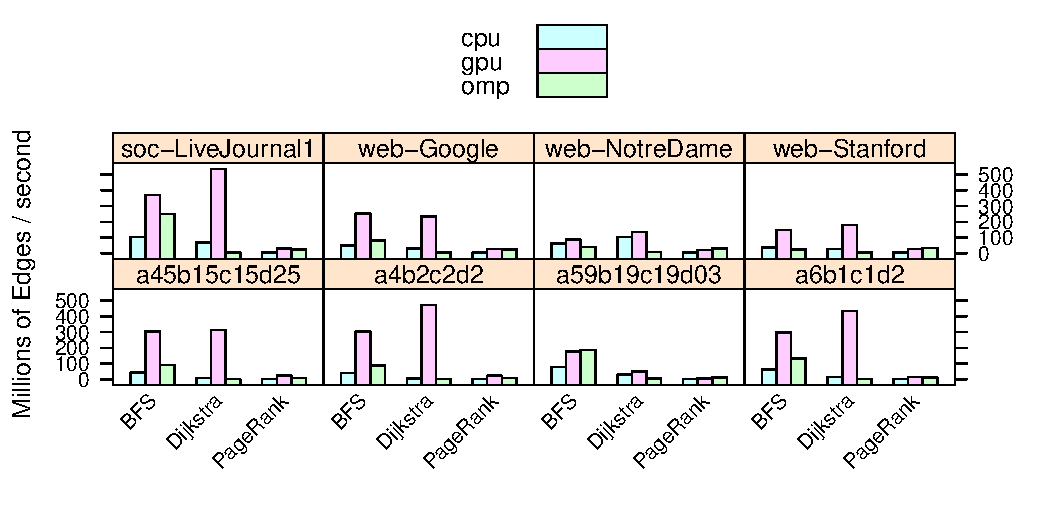
\includegraphics{figures/edges_per_second.pdf}}}
\caption{Processing ratio}
\label{fig:rate}
\end{center}
\end{figure*}

Figure \ref{fig:rate} shows the processing rate (i.e., edges per second) for each combination of algorithm, workload, and platform. There are two important aspects to highlight. First, the GPU implementation achieves superior performance in the majority of scenarios; second, the observed performance variation from one scenario to another suggests that graph characteristics play an important role in the attainable performance. The next paragraphs discuss these points in turn.

In the set of real-world graphs (top line), the GPU implementation achieves a peak performance of approximately $10^5$ edges/s (Dijkstra, LiveJournal). It is important to note that this is an estimation of the processing rate an accelerator (in a hybrid system) would be be to deliver compared to alternative platforms. In practice, the GPU would be primarily used to offload processing from the host processors. Therefore, such hybrid platform has the potential to deliver even higher performance when compared to the referred CPU and OpenMP implementations evaluated above.

Although the performance levels above provide evidence that hybrid platforms are attractive for graph processing, we also observe some variations in the relative performance across workloads for the same algorithm. More specifically, the relative performance PageRank on GPU and OpenMP platforms seems to depend on the workload. This is illustrated by the processing rates achieved on {\em web-Google} and {\em liveJournal} compared to {\em web-NotreDame} and {\em web-Stanford}. Similarly, the relative performance is not consistent across the R-MAT graphs. 

One potential source for these inconsistencies is the work imbalance across threads, which is a result of non-uniform connectivity across the nodes in the graph (e.g., node degree). More specifically, the hypothesis is that node degree imbalance will cause threads divergence in the GPU-implementations and hinder its performance. 

To test this hypothesis, we characterize the node degree distribution of each graph in the workload and correlate it with the achieved performance. The characterization considers two metrics of the concentration of a distribution: Kurtosis; and the $\alpha$ coefficient of a fitted power-law (i.e., the slope of the line on the log-log plot of the node degree distribution) (see Table~\ref{tab:kurtosis}). 

\begin{table}[ht]
\centering
\begin{tabular}{l|r|r}
Name              & Kurtosis   & $\alpha$ \\\hline
Web (Google)      & 142.20   & 1.47    \\\hline
Web (NotreDame)   & 2088.50  & 1.45    \\\hline
Web (Stanford)    & 57.60    & 1.45    \\\hline
OSN (LiveJournal) & 29667.00 & 1.40    \\\hline
A45               & 132.02  & 1.51    \\\hline
A4                & 167.50   & 1.51    \\\hline
A59               & 73959.00 & 1.56    \\\hline
A6                & 3660.10  & 1.55     \\\hline
\end{tabular}
\caption{Approximate values for the node degree distribution characteristics metrics.}
\label{tab:kurtosis}
\end{table}
            
If there is a negative correlation between the characteristics of the node degree distribution, as represented by the kurtosis and the $\alpha$ coefficient, the influence of the node degree distribution imbalance on the performance is confirmed. 

\begin{table}[ht]
\centering
\begin{tabular}{l|r|r}
Name     & $\rho(kurtosis,e)$ & $\rho(\alpha,e)$ \\\hline
BFS      & -0.2049       &  0.2649 \\\hline
Dijkstra & -0.5921       & -0.0869 \\\hline
PageRank & {\bf -0.6632} & {\bf -0.7331} \\\hline
\end{tabular}
\caption{Person's correlation coefficient between processing rate of GPU implementations and the workload characteristics.}
\label{tab:corr}
\end{table}

Table~\ref{tab:corr} contains the the Person's correlation coefficient $\rho$ between the observed performance (i.e., edges/s $= e$) of each GPU implementation and the workload characteristics. These results confirm our intuition that the inconsistencies in performance observed on the GPU implementation PageRank is due to relatively few high-degree nodes. The existence of these nodes translate into a {\em peaky} node degree distribution (i.e., a large value for both $\alpha$ and kurtosis). In turn, such graph workload imply less parallelism in the application, as some threads will have much more work to process, while others finish early and stay idle. 

Although these correlations provide initial support to the intuition that the node degree distribution characteristics influence the observed performance of graph algorithms on GPU, these results should be taken with caution. A more comprehensive study that includes a larger sample of both real-world and synthetic graphs together with the application of complementary data analysis approaches (e.g., regression analysis, and principal component analysis) is necessary to provide a statistically grounded conclusion. Nevertheless, these preliminary results show that we are on the right direction.

Finally, it is worth noting the poor performance of the OpenMP implementation of Dijkstra's algorithm: the processing rate is consistently lower than that for its sequential version. The reason for this bad performance is granted to a naive synchronization approach adopted in the current OpenMP implementation, threads use a global lock over the entire set of vertices, when only a lock that protects only the neighbors of a given vertex that are processed by the current thread. A simple solution that trades run time for a larger memory footprint consists of having one lock per vertex in the graph. The evaluation of such implementation is left for future work.
